\subsection{Results of the Measurement}
\label{sec:analysis_1:results}

Before we introduce measurement results, i.e., the different metrics and the abstract operations' distribution,  we introduce the sample's composition, i.e., the data cleaning results. 
\begin{figure}[t]
    \centering
        \begin{tikzpicture}
        \pie[ 
        /tikz/every pin/.style={align=left},
        radius=3.5,
        sum=auto,
        text=pin,
        % color={orange!100,orange!50,yellow!50,cyan!50,blue!50},
        before number=\phantom, 
        after number=
        ]{
        50/$\textbf{No top-level}$ \\$\textbf{resources}$ \\ (50 APIs $\vert$ 2.42\%),
        372/$\textbf{Toy APIs}$ \\(372 APIs $\vert$ 17.98\%) ,
        163/$\textbf{Evaluation tool}$  \\ $\textbf{cannot process}$ \\ (163 APIs $\vert$  7.88\%),
        303/$\textbf{OpenISBT throws}$ \\$\textbf{an exception}$ (303 APIs $\vert$ 14.64\%),
        1181/$\textbf{Included in}$ \\ $\textbf{analysis}$ \\ (1181 APIs $\vert$  57.08\%)
        }
        \end{tikzpicture}
    \caption{Distribution of the OpenAPI documents by applied data cleaning components}
    \label{fig:pie_chart:shares_of_removed_apis_before_extention}
\end{figure}
\FloatBarrier
Figure \ref{fig:pie_chart:shares_of_removed_apis_before_extention} shows it as a pie chart. We pass the evaluation tool 2069 OpenAPI documents.
We identify 372 OpenAPI documents, which describe toy APIs. We consider 297 of them as toy APIs as they are too short, i.e., they have less than 100 LOC. The other 75 documents are templates, which SwaggerHub provides. Also, we detect 163 OpenAPI documents, which the evaluation tool cannot process because they define general path-properties. 

We also detect 303 OpenAPI documents, which openISBT cannot handle without throwing an exception. Furthermore, we detect 50 OpenAPI documents, which openISBT cannot handle since the documents only define operations on nested resources.

We know by observation that the sample contains 158 template documents, but as we mention above, we only identify 75 template documents. Furthermore, we do not identify any document with a missing paths-property, but we know by observation that the sample contains 15 such documents. Interdependencies mentioned in section \ref{sec:eval_tool:design_and_architecture} are the reason for this. However, we ensure that these interdependencies do not affect results correctness. 

\begin{figure}
\centering
\begin{subfigure}[t]{.48\textwidth}
  \centering
%%%%%%%%%%%%%%%%%%%%%%%%%%%%%%%%%%%%%%%%%%% 
%%%%%%%%%%%%%%% OPERATIONS %%%%%%%%%%%%%%%%
%%%%%%%%%%%%%%%%%%%%%%%%%%%%%%%%%%%%%%%%%%% 
    \begin{tikzpicture}
        \pie[ 
            /tikz/every pin/.style={align=left},
            sum=auto,
            radius=2,
            text=pin,
            rotate=70 ,
            % before number=\phantom,
            % after number=,
            color={red!70,blue!70}
            ]{
            3301/$\textbf{Not supported}$\\ (24.8\%),
            10009/$\textbf{Supported}$\\ (75.2\%)
            }
    \end{tikzpicture}
%%%%%%%%%%%%%%%%%%%%%%%%%%%%%%%%%%%%%%%%%%% 
%%%%%%%%%%%%%%%%%%%%%%%%%%%%%%%%%%%%%%%%%%% 
%%%%%%%%%%%%%%%%%%%%%%%%%%%%%%%%%%%%%%%%%%% 
  \caption{OpenISBT matches 10009 of 13310 operations across all APIs.}
  \label{fig:analysis1_sub_pie_coverage_sup_operations_main}
\end{subfigure}%
\hfill
\begin{subfigure}[t]{.48\textwidth}
  \centering
%%%%%%%%%%%%%%%%%%%%%%%%%%%%%%%%%%%%%%%%%%% 
%%%%%%%%%%%%%%%%%% APIs %%%%%%%%%%%%%%%%%%%
%%%%%%%%%%%%%%%%%%%%%%%%%%%%%%%%%%%%%%%%%%% 
    \begin{tikzpicture}
        \pie[ 
            /tikz/every pin/.style={align=left},
            sum=auto,
            radius=2,
            text=pin,
            % before number=\phantom,
            % after number=,
            color={red!70,blue!70}
            ]{
            692/$\textbf{Not fully}$ \\$\textbf{supported}$ \\ (58.6\%),
            489/$\textbf{Fully supported}$\\ (41.4\%)
            }
    \end{tikzpicture}
%%%%%%%%%%%%%%%%%%%%%%%%%%%%%%%%%%%%%%%%%%% 
%%%%%%%%%%%%%%%%%%%%%%%%%%%%%%%%%%%%%%%%%%% 
%%%%%%%%%%%%%%%%%%%%%%%%%%%%%%%%%%%%%%%%%%% 
  \caption{For 489 of 1181 APIs openISBT matches all operations on top-level resources.}
  \label{fig:analysis1_sub_pie_coverage_full_sup_apis_main}
\end{subfigure}%
%\caption{Both coverages we determined for a set of 1181 APIs and 13310 operations}
\caption{Coverage metrics for a set of 1181 OpenAPI documents including 13310 service operations}
\label{fig:analysis1_pie_both_criteria_main}
\end{figure}

Figure \ref{fig:analysis1_pie_both_criteria_main} shows two pie charts visualizing the coverage metrics.
Pie chart \ref{fig:analysis1_sub_pie_coverage_sup_operations_main} shows the shares of supported and unsupported service operations. Supported service operations can be successfully matched to an abstract operation by the openISBT matching tool, and unsupported operations cannot. In other words, the share of the supported operation in the pie chart is the metric $p_{operations}$. The chart mainly expresses that openISBT can match 10009 of 13310 service operations to abstract operations, i.e., the coverage $p_{operations}$ is equal to $75.2\%$.

Figure \ref{fig:analysis1_sub_pie_coverage_full_sup_apis_main} shows the shares of fully supported APIs as a pie chart. 
Fully supported means that openISBT supports all service operations an API defines.
Therefore, the relative share of the fully supported APIs of 41.4\% is the coverage metric $p_{APIs}$.

The cleaned sample of documents both pie charts refer to includes 1181 OpenAPI documents and 13310 service operations on top-level resources. 

\begin{figure}[t]
    \centering
        \begin{tikzpicture}
        \pie[ /tikz/every pin/.style={align=left},
        sum=auto,
        radius=3.5,
        text=pin,
        color={blue!70,blue!70,blue!70,blue!70,red!70,blue!70},
        before number=\phantom,
        after number=]{
        4706/$\textbf{CREATE}$ \\ (4706 oper. $\vert$ 35.35\%),
        1860/$\textbf{READ}$ \\ (1860 oper. $\vert$ 13.97\%),
        1237/$\textbf{SCAN}$ \\ (1237 oper. $\vert$ 9.29\%),
        1194/$\textbf{UPDATE}$ \\ (1194 oper. $\vert$ 8.97\%),
        3301/$\textbf{UNDEFINED}$ \\ (3301 oper. $\vert$ 24.80\%),
        1012/$\textbf{DELETE}$ \\ (1012 oper. $\vert$ 7.60\%)
        }
        \end{tikzpicture}
    \caption{Distribution of the service operations by matched abstract operations}
    \label{fig:analysis1:pie_chart_shares_of_operation_types}
\end{figure}
Beyond calculating coverage metrics, we also determine the distribution of the abstract operations, i.e.,  how often openISBT matches each abstract operation. Figure \ref{fig:analysis1:pie_chart_shares_of_operation_types} shows the shares of each abstract operation. 
If a service operation is not supported, then the abstract operation is undefined yet. 
Therefore, the slice UNDEFINED contains all the unsupported service operations.
We also notice that openISBT matches 4706 service operations (35.35\%) to the abstract operation CREATE, which is significantly higher than the other operations. 


\subsection{The Larger Scope of Applicability}
\label{sec:analysis1:larger_context_of_applicability}
Determining the results above, we set focus on discovering missing abstract operations. Therefore, we ignore documents and service operations if openISBT does not support them for other reasons than undiscovered abstract operations. Figure \ref{fig:analysis1_pie_both_criteria_all_factors} visualizes the metrics as figure \ref{fig:analysis1_pie_both_criteria_main} but reflects any aspect of applicability.

\begin{figure}[!hb]
\centering
\begin{subfigure}[t]{.48\textwidth}
  \centering
%%%%%%%%%%%%%%%%%%%%%%%%%%%%%%%%%%%%%%%%%%% 
%%%%%%%%%%%%%%% OPERATIONS %%%%%%%%%%%%%%%%
%%%%%%%%%%%%%%%%%%%%%%%%%%%%%%%%%%%%%%%%%%% 
    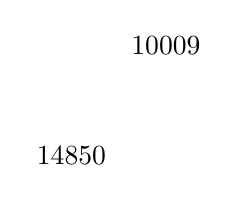
\begin{tikzpicture}
        \pie[ 
            /tikz/every pin/.style={align=left},
            sum=auto,
            radius=2,
            text=pin,
            rotate=120,
            before number=\phantom,
            after number=,
            color={red!70,blue!70}
            ]{
            14.850/$\textbf{Not supported}$\\ (59.7\%),
            10.009/$\textbf{Supported}$\\ (40.3\%)
            };
            \node[] at (0.6, 0.7){10009};
            \node[] at (-0.6,-0.7){14850};
    \end{tikzpicture}
%%%%%%%%%%%%%%%%%%%%%%%%%%%%%%%%%%%%%%%%%%% 
%%%%%%%%%%%%%%%%%%%%%%%%%%%%%%%%%%%%%%%%%%% 
%%%%%%%%%%%%%%%%%%%%%%%%%%%%%%%%%%%%%%%%%%% 
  \caption{OpenISBT matches 10009 of 24859 Operations across all APIs.}
  \label{fig:analysis1_sub_pie_coverage_sup_operations_all_factors}
\end{subfigure}%
\hfill
\begin{subfigure}[t]{.48\textwidth}
  \centering
%%%%%%%%%%%%%%%%%%%%%%%%%%%%%%%%%%%%%%%%%%% 
%%%%%%%%%%%%%%%%%% APIs %%%%%%%%%%%%%%%%%%%
%%%%%%%%%%%%%%%%%%%%%%%%%%%%%%%%%%%%%%%%%%% 
    \begin{tikzpicture}
        \pie[ 
            /tikz/every pin/.style={align=left},
            sum=auto,
            radius=2,
            text=pin,
            rotate=90,
            % before number=\phantom,
            % after number=,
            color={red!70,blue!70}
            ]{
            1159/$\textbf{Not fully}$ \\$\textbf{supported}$ \\ (75.6\%),
            375/$\textbf{Fully supported}$\\ (24.4\%)
            }
    \end{tikzpicture}
%%%%%%%%%%%%%%%%%%%%%%%%%%%%%%%%%%%%%%%%%%% 
%%%%%%%%%%%%%%%%%%%%%%%%%%%%%%%%%%%%%%%%%%% 
%%%%%%%%%%%%%%%%%%%%%%%%%%%%%%%%%%%%%%%%%%% 
  \caption{For 375 of 1534 APIs openISBT matches all operations.}
  \label{fig:analysis1_sub_pie_coverage_full_sup_apis_all_factors}
\end{subfigure}%
\caption{Coverage metrics for a set of 1534 OpenAPI documents including 24859 service operations}
\label{fig:analysis1_pie_both_criteria_all_factors}
\end{figure}


Therefore, it considers 1534 OpenAPI documents, which define 24859 service operations on top-level resources and nested resources.
If openISBT cannot process an OpenAPI document without exception, or the OpenAPI document only defines nested resources, we count it as $p_i=0$. Figure  \ref{fig:analysis1_sub_pie_coverage_sup_operations_all_factors} shows a  much smaller coverage of 40.3\% for the supported service operations.
Also, figure \ref{fig:analysis1_sub_pie_coverage_full_sup_apis_all_factors} shows a smaller coverage of 24.4\% for the fully supported APIs. 
